%%% PREAMBLE - Do not touch %%%%%%%%%%%%%%%%%%%%%%%%%%%%%%%%%%%%%%%%%%%%%%%%%%%%%%
\documentclass[10pt,twocolumn,letterpaper]{article}
\usepackage[utf8]{inputenc}
\usepackage[portuges,brazil,english]{babel}
\usepackage{model}
\usepackage{times}
\usepackage{epsfig}
\usepackage{graphicx}
\usepackage{amsmath}
\usepackage{amssymb}
\usepackage{color}
\usepackage[pagebackref=true,breaklinks=true,letterpaper=true,colorlinks,bookmarks=false]{hyperref}

\cvprfinalcopy % *** Uncomment this line for the final submission
\def\httilde{\mbox{\tt\raisebox{-.5ex}{\symbol{126}}}}
\ifcvprfinal\pagestyle{empty}\fi

\newcommand{\TODO}[1]{TODO: #1}
\newcommand{\CITEONE}[2]{\mbox{#1 \cite{#2}}}
\newcommand{\CITETWO}[3]{\mbox{#1 and #2 \cite{#3}}}
\newcommand{\CITEN}[2]{\mbox{#1 et al. \cite{#2}}}

%%% Paper beginning %%%%%%%%%%%%%%%%%%%%%%%%%%%%%%%%%%%%%%%%%%%%%%%%%%%%%%%%%%%%%%
\begin{document}

%%% Title and authors %%%%%%%%%%%%%%%%%%%%%%%%%%%%%%%%%%%%%%%%%%%%%%%%%%%%%%%%%%%%
\title{MC886 - Trabalho prático individual}
\author{Guilherme P. Gonçalves (RA 091429)}

%%% Abstract %%%%%%%%%%%%%%%%%%%%%%%%%%%%%%%%%%%%%%%%%%%%%%%%%%%%%%%%%%%%%%%%%%%%%
\maketitle
\begin{abstract}
Este trabalho propõe um algoritmo de aprendizado online dos recursos carregados por páginas da Internet, como \emph{scripts} e imagens, e agrupamento de recursos similares carregados por páginas sob uma mesma origem. Se disponíveis de antemão no momento em que o usuário requisita uma página, tais informações podem ser utilizadas pelo navegador para tomar ações especulativas, como pré-resolução DNS de URLs de recursos, tornando o carregamento da página mais rápido. O algoritmo proposto foi avaliado experimentalmente no navegador Firefox.
\end{abstract}

%%% Introduction %%%%%%%%%%%%%%%%%%%%%%%%%%%%%%%%%%%%%%%%%%%%%%%%%%%%%%%%%%%%%%%%%
\section{Introdução}

A performance de navegadores web modernos depende de diversos fatores, como as velocidades de \emph{parsing} de documentos HTML, ou de execução de Javascript. No entanto, a camada de rede possui importância especial, visto que pouco se pode avançar nas demais etapas do carregamento de uma página enquanto os dados ainda são trazidos, potencialmente com vários milissegundos de atraso, através da rede.

Uma área de possível otimização da camada de rede envolve fazer com que o navegador aprenda os padrões de acesso a recursos de uma página. Dessa forma, quando uma página é requisitada, alguma ações preditivas podem ser tomadas pelo navegador para agilizar a busca de recursos como imagens ou arquivos de \emph{script}. Tais otimizações são particularmente importantes em ambientes móveis, com conexões 3G e 4G, que possuem alto \emph{round trip time} (RTT), fazendo com que mesmo o estabelecimento de uma conexão TCP a um recurso, antes do envio de dados, atrase significativamente o carregamento de uma página.

O navegador Google Chrome possui um algoritmo \cite{ChromeLearning:2013:Online} que explora essa ideia, e executa ações como pré-resoluções de DNS, pré-conexões, ou mesmo requisições especulativas de recursos e pré-renderização de páginas. Recentemente um outro algoritmo similar foi implementado no navegador Firefox \cite{BugzillaSeer:2013:Online}, embora sem envolver ações mais agressivas (e, portanto, com implicações mais sérias para a privacidade do usuário) como as requisições especulativas.

O algoritmo implementado no Firefox opera, em linhas gerais, sobre páginas isoladas: para cada página, tendo-se os recursos que ela já requisitou no passado, a razão do número de vezes em que um recurso foi acessado pela página pelo número de vezes que a página foi acessada dá um valor de \emph{confiança} de que aquele recurso será necessário no próximo carregamento da página. Dependendo do valor da confiança, e da data dos últimos acessos da página e do recurso, o navegador toma ações como pré-resolução de DNS  (baixa confiança) ou pré-conexão (alta confiança).

Este trabalho explora uma abordagem diferente, em que todos os recursos acessados por páginas sob uma mesma origem são considerados de forma a encontrar grupos de recursos com padrões de acessos semelhantes. Quando uma página é requisitada, os grupos de recursos que melhor descrevem o comportamento passado da página são utilizados em ações preditivas. Dessa forma, caso duas páginas sejam visitadas em sucessão com frequência, por exemplo, seus recursos tendem a ser acessados de forma semelhante, e a navegação para uma delas causa a tomada de ações preditivas não apenas para os recursos dela, mas também para os da outra, potencialmente agilizando ambos os acessos.

A Seção \ref{sec-algorithm-highlevel} discute algumas das decisões iniciais que nortearam este trabalho e descreve em alto nível o algoritmo proposto, enquanto a seção \ref{sec-algorithm-detail} detalha seu funcionamento. A Seção \ref{sec-experiments} traz resultados de testes desse algoritmo em comparação com o navegador Firefox sem nenhum algoritmo de aprendizagem, e com o algoritmo atual.

\section{Descrição geral do algoritmo}
\label{sec-algorithm-highlevel}

Desde o início, tomou-se como prioridade explorar o problema de predição de recursos sob um ângulo completamente diferente daquele utilizado pelos navegadores Chrome e Firefox. Dessa forma, enquanto estes algoritmos buscam otimizar o carregamento de uma página utilizando informações de acessos de recursos daquela página, o algoritmo aqui desenvolvido utiliza informações mais gerais da origem da página para otimizar a navegação através de um conjunto de páginas.

Além disso, o algoritmo atual no Firefox possui um número alto de constantes e parâmetros, o que, ao mesmo tempo que lhe confere flexibilidade, também o torna complexo e torna necessário um esforço de engenharia para encontrar a melhor combinação de valores para esses parâmetros. Buscou-se, no desenvolvimento deste algoritmo, expor, se possível, um número menor de parâmetros ajustáveis, facilitando assim a avaliação experimental.

O algoritmo proposto é essencialmente por uma aplicação de clusterização sobre os recursos carregados por páginas sob uma mesma origem. A clusterização acontece em dois níveis: primeiramente, todos os recursos sob uma determinada origem são agrupados em \emph{clusters}; a seguir, cada cluster é dividido em \emph{subclusters}.

Uma vez calculados os agrupamentos, quando uma página já conhecida é carregada, escolhem-se como predição os recursos nos \emph{clusters} e \emph{subclusters} que melhor cobrem o conjunto de recursos requisitados por aquela página na última vez em que foi carregada. Caso a página não seja conhecida, isto é, jamais tenha sido visitada pelo usuário, ainda é possível inferir a partir dos \emph{clusters} quais recursos são mais importantes para todas as páginas sob aquela origem, e possivelmente agir sobre eles. Para este trabalho, foi implementada apenas uma heurística simples para identificar esses recursos. Este caso é de particular interesse, pois o algoritmo atual do Firefox não toma ação alguma para páginas desconhecidas. 

Como as informações de recursos e páginas mudam à medida que o usuário navega, é necessário que o algoritmo seja \emph{online}. Para isso, basta recalcular periodicamente o agrupamento, utilizando dados pertencentes a uma determinada janela de tempo no passado e descartando dados antigos demais.

Enquanto está sendo utilizado, o navegador Firefox guarda algumas informações que são utilizadas por seu algoritmo de predição: \emph{timestamp} de acesso de cada página e recurso, quais páginas carregaram quais recursos, e número de acessos a cada página e recurso. Como hipótese simplificadora para o desenvolvimento deste trabalho, optou-se por utilizar essas mesmas informações para descrever recursos.

\section{Descrição detalhada do algoritmo}
\label{sec-algorithm-detail}

Sejam $P$ o conjunto de páginas conhecidas para uma dada origem, $r$ um recurso e $P_{r} \subseteq P$ o conjunto das páginas que requisitaram aquele recurso dentro da janela de tempo de tamanho $W = now() - W_0$ no passado. Sejam $T(r)$,  $T(p)$, $H(r)$ e $H(p)$ a data do último acesso e o número de acessos ao recurso $r$ e à página $p$, respectivamente. No caso dos recursos, são levados em conta todos os acessos de páginas sob a mesma origem, ou seja, $H(r)$ é a soma do número de acessos de todas as páginas de $P_{r}$ a $r$, e $T(r)$ é a data (expressa em uma \emph{timestamp} Unix) do mais recente desses acessos.

Cada recurso é então descrito pelo vetor bidimensional dado pela Equação \ref{fv-eqn}:

\begin{equation}
\label{fv-eqn}
v_{r} = \left( \frac{T(r) - W_0}{now() - W_0}, \frac{H(r)}{b_{o} + \sum_{p \in P_{r}} H(p)} \right)
\end{equation}

Assim, uma das componentes do \emph{feature vector} é simplesmente o tempo de acesso mais recente do vetor, normalizado pelo tamanho da janela de tempo $W$. O tamanho da janela, embora possa ser considerado um parâmetro, pouco influi no resultado do algoritmo quando grande o suficiente para evitar descarte excessivo de dados (note que acessos anteriores ao começo da janela $W_0$ são desconsiderados). Para o desenvolvimento deste trabalho, utilizou-se uma janela de duas semanas. Esta primeira componente dá uma medida de importância global do recurso dentro daquela origem, visto que qualquer acesso a ele por qualquer página é suficiente para atualizar seu tempo de acesso mais recente.

A segunda componente do vetor é uma quantidade de acessos relativa, que expressa a importância de um determinado recurso para as páginas que o requisitam. No numerador, tem-se apenas o número total de acessos àquele recurso por todas as páginas do host, $H(r)$. No denominador, têm-se as quantias $\sum_{p \in P_{r}} H(p)$, o número total de acessos das páginas em $P_{r}$, e $b_{o}$, um \emph{bias} específico para aquela origem.

A inclusão de $b_{o}$ diferencia o caso em que um recurso $r$ possui, por exemplo, 100 acessos por 100 páginas diferentes sob uma mesma origem, cada uma com um acesso, do caso em que $r$ foi acessado apenas uma vez por uma única página. Supondo $b_{o}$ igual a zero, em ambos os casos a segunda componente do vetor de $r$ seria igual a $1$, embora seja desejável reconhecer que $r$ é bem mais importante no contexto da origem considerada no primeiro caso do que no segundo.

Sendo assim, toma-se como $b_{o}$ a moda do número de acessos das páginas daquela origem:

\begin{equation}
b_{o} = mode(H(p), \forall p \in P)
\end{equation}

Portanto, se $b_{o}$ e $\sum_{p \in P_{r}} H(p)$ são próximos, então aquele recurso provavelmente foi acessado apenas por poucas páginas, com números comuns de acessos (próximos de $b_{o}$), ou por muitas páginas, cada uma delas com número anormalmente baixo de acessos. De qualquer forma, conclui-se que aquele recurso não é importante, e seu vetor é penalizado. Note que esta distinção não leva em conta o número de páginas que acessam um recurso -- seja o somatório de $H(p)$ alto devido a um grande número de acessos a um recurso por uma única página ou devido a vários acessos por várias páginas, a importância do recurso permanece a mesma.

Os vetores de todos os recursos são então agrupados utilizando o algoritmo Kmeans com distância Euclidiana. Durante o desenvolvimento do algoritmo proposto, utilizou-se como \emph{dataset} auxiliar dados de navegação coletados pelo Firefox durante duas semanas no YouTube. Vários dos parâmetros do algoritmo proposto, inclusive a escolha do valor de K na aplicação do Kmeans, foram derivados de experimentos nesse conjunto de dados.

Para a escolha do valor de K, utilizou-se a regra do cotovelo. Conforme mostra a Figura \ref{fig-youtube-elbow}, a distorção (somatório da diferença quadrada entre cada vetor e o centróide de seu \emph{cluster}) tem maior redução para K próximo de 10. Foi tomado, portanto, esse valor fixo para o algoritmo final, embora uma estratégia adaptativa que escolha um valor menor com menos dados possa ser desejável no futuro. Cada cluster é então dividido novamente em 5 \emph{subclusters}. Esse processo é feito para cada um dos hosts conhecidos pelo navegador.

\begin{figure}
	\begin{center}
     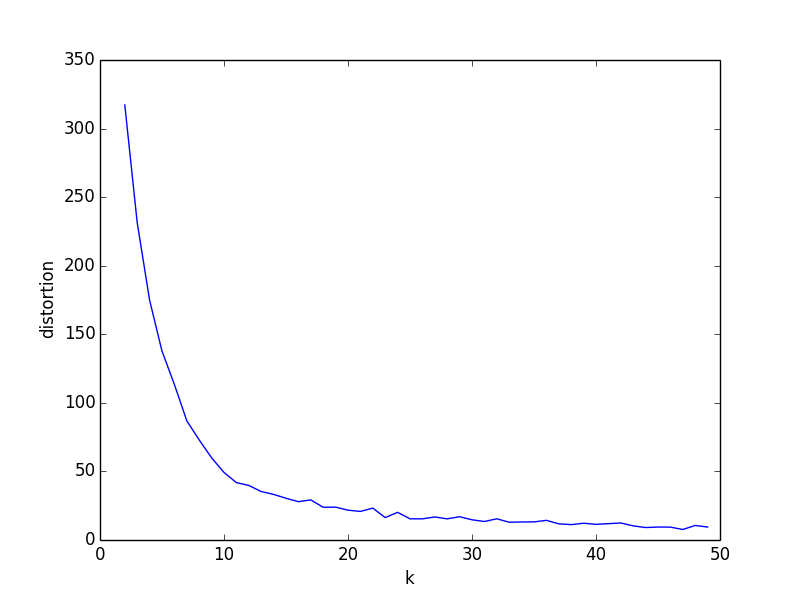
\includegraphics[width=0.99\columnwidth]{pics/youtube_elbow.png}
    \caption{Distorção em função de K para o dataset do YouTube.}
    \label{fig-youtube-elbow}   
	\end{center} 
\end{figure}

Quando uma página conhecida é visitada, então, o algoritmo consiste em computar o conjunto $R_{explicit}$ de recursos carregados explicitamente pela página em seu último acesso (denominados recursos explícitos), utilizando $T(r)$ e $T(p)$, e então selecionar os 4 clusters que contém o maior número de recursos de $R_{explicit}$. O número 4 foi escolhido porque, experimentalmente, observou-se que 3 clusters eram suficientes para cobrir acima de 90\% dos $R_{explicit}$ de quase todas as páginas no \emph{dataset} do YouTube, e o cluster a mais serve para fornecer a liberdade para que sejam selecionados clusters com recursos de outras páginas.

Dos 20 subclusters que compõem esses 4 clusters, são selecionados para o conjunto de predição $R_{selected}$ os 15 que melhor cobrem $R_{explicit}$, desde que sua seleção não faça com que $R_{selected}$ tenha tamanho maior do que 50\% do tamanho de $R_{explicit}$. O valor 50\% é um parâmetro que controla a agressividade do algoritmo ao fazer suas predições. O conjunto de recursos para os quais serão tomadas ações preditivas é, então:

\begin{equation}
R_{predicted} = R_{explicit} \cup R_{selected}
\end{equation}

Para páginas não conhecidas, são selecionados simplesmente os 15 subclusters mais próximos do ponto $(1, 1)$, dentre os 4 clusters também mais próximos desse ponto.

A Figura \ref{fig-youtube-explicit-vs-predicted} ilustra o crescimento linear o tamanho de $R_{predicted}$ em função do tamanho de $R_{explicit}$ para cada página nos dados retirados do YouTube, mostrando o funcionamento do controle da agressividade do algoritmo.

\begin{figure}
	\begin{center}
     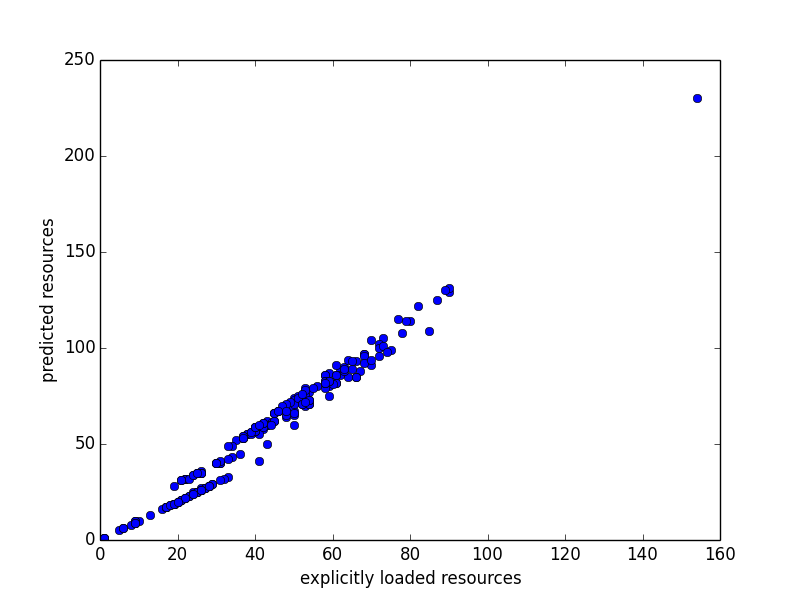
\includegraphics[width=0.99\columnwidth]{pics/youtube_explicit_vs_predicted.png}
    \caption{Crescimento de $R_{predicted}$ em função do tamanho de $R_{explicit}$ nos dados do YouTube.}
    \label{fig-youtube-explicit-vs-predicted}   
	\end{center} 
\end{figure}

A Figura \ref{fig-youtube-explicit-predicted-over-predicted} é um histograma da fração de $R_{explicit}$ em $R_{predicted}$ nas páginas do YouTube, mostrando como, embora essa fração seja limitada inferiormente, para a maior parte das páginas ainda é possível obter predições substancialmente maiores do que apenas $R_{explicit}$. 

\begin{figure}
	\begin{center}
     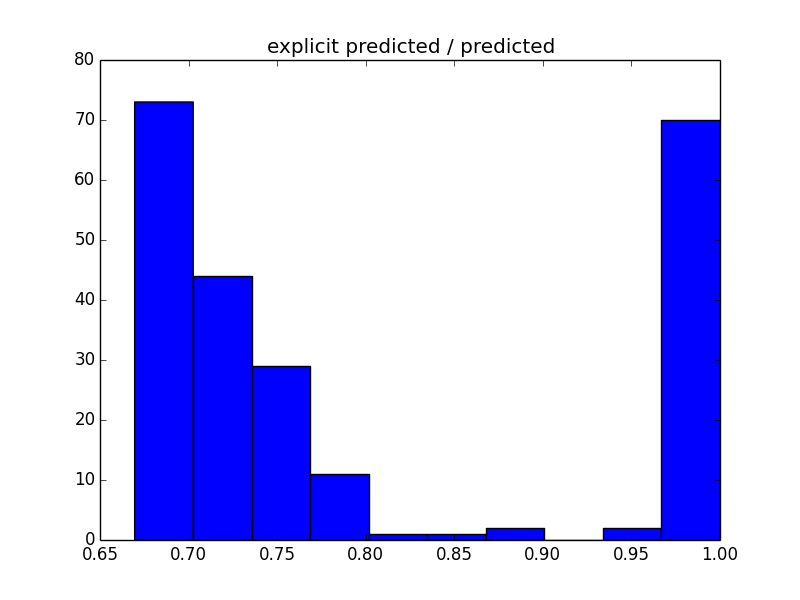
\includegraphics[width=0.99\columnwidth]{pics/youtube_explicit_predicted_over_predicted.png}
    \caption{Crescimento de $R_{predicted}$ em função do tamanho de $R_{explicit}$ nos dados do YouTube.}
    \label{fig-youtube-explicit-predicted-over-predicted}   
	\end{center} 
\end{figure}

\section{Resultados experimentais}
\label{sec-experiments}

Esta seção contém os resultados da avaliação experimental do algoritmo proposto.

A metodologia dos testes consistiu em visitar algumas páginas por quatro dias, de forma a coletar dados de treinamento necessários para as predições, e então submeter o navegador a rodadas do WebPageTest \cite{WebPageTest:2013:Online}, uma ferramenta que permite medir diversas estatísticas durante o carregamento de uma página. Em particular, para estes testes, tomou-se como métrica de qualidade das predições o SpeedIndex \cite{SpeedIndex:2013:Online}, uma medida aproximada do tempo de carregamento da página em milisegundos conforme percebido pelo usuário. Dessa forma, um bom algoritmo de predição deve resultar em uma redução do SpeedIndex.

Cada execução do WebPageTest envolveu 20 acessos a uma página em velocidade de conexão 3G.  Embora o WebPageTest também execute acessos repetidos à página (ou seja, a cada execução têm-se resultados de 20 primeiros acessos e 20 acessos repetidos), a fim de minimizar a interferência do \emph{cache} sobre os testes, e também porque os dados necessários para a predição já estavam presentes no navegador (ou seja, não se buscava aprendizado durantes os testes), foi considerado apenas o SpeedIndex dos primeiros acessos.

Para cada teste, foram comparadas três variantes do Firefox: \emph{kmeans}, que utiliza o algoritmo aqui proposto, \emph{seer}, que utiliza o algoritmo já existente no navegador, e \emph{noseer}, que não toma nenhum tipo de ação preditiva, servindo como \emph{baseline}. Para a variante \emph{kmeans}, a única ação preditiva tomada foi a pré-conexão para todos os recursos preditos para uma página. Todas as variantes utilizaram os mesmos dados de treinamento durante os testes.

Cabe notar ainda dois problemas observados na metodologia de testes.

Primeiramente, por restrições da infraestrutura, os testes foram executados sobre uma conexão direta com a Internet (e não, por exemplo, usando WebPageReplay \cite{WebPageReplay:2013:Online}). Além de prejudicar a reprodutibilidade dos resultados, visto que as páginas usadas no teste estão sujeitas a mudanças, isso faz também com que os experimentos sejam afetados por oscilações normais na rede. No entanto, na medida em que os experimentos foram todos executados juntos, pode-se considerar pequena a influência desses fatores sobre o resultado final.

Além disso, como a coleta inicial de dados e os testes no WebPageTest ocorreram em computadores diferentes, algumas pequenas diferenças entre essas máquinas causaram o carregamento de recursos diferentes, porém equivalentes, pela mesma página. Por exemplo, diferenças de resolução nas máquinas fazem com que imagens que diferem apenas no tamanho (e na URL) sejam acessadas pela mesma página no treinamento e no teste. Dado que as predições não causam \emph{download} dos recursos, mas apenas pré-conexão ao servidor responsável por eles, isso em geral não afeta os resultados experimentais. No entanto, a análise da acurácia das predições fica prejudicada, visto que a simples comparação entre as URLs dos recursos preditos e efetivamente carregados durante o teste considera errada uma predição que estaria correta caso o treinamento tivesse sido feito na mesma máquina que o teste. Dessa forma, as taxas de acerto desta seção devem ser tomadas como limitantes inferiores apenas.

A Tabela \ref{tbl-turing} contém o SpeedIndex para a primeira visualização no teste \emph{turing}, que consiste em acessar o artigo sobre Alan Turing na Wikipedia. Trata-se de um teste simples para exercitar os algoritmos em uma página que sofre poucas modificações com o tempo.

\begin{table}
\begin{center}
\begin{tabular}{l*{6}{c}r}
\hline
Algoritmo & Mediana & Média & Desvio padrão \\
\hline
kmeans & 20.115,00 & 19.299,30  & 2.439,00 \\
noseer & 22.968,00 & 22.838,50 & 4.954,00 \\
seer & 25.000,00 & 22.575,15 & 2.471,00 \\
\hline
\end{tabular}
\end{center}
\caption{SpeedIndex para o experimento turing.}
\label{tbl-turing}
\end{table}

Assumindo distribuição Gaussiana da média, observa-se que a média do algoritmo \emph{kmeans} ficou $3,19$ desvios padrão abaixo do \emph{noseer}. O algoritmo \emph{seer}, em comparação, ficou apenas $0,23$ desvios padrão abaixo do \emph{baseline}. Neste teste, ao menos $33,82 \%$ das predições feitas pelo algoritmo \emph{kmeans} estavam de fato corretas (isto é, foram de fato feitas no teste com a mesma URL), e essas predições corretas compõem ao menos $53,49 \%$ de todas as requisições de recursos feitas no teste. De todas as requisições feitas, $58,14 \%$ eram conhecidas, ou seja, já haviam sido feitas pela página durante o treinamento. Isso evidencia que, embora não seja necessariamente preciso prever com sucesso grande parte das requisições conhecidas para se obter bons resultados, ainda pode haver espaço para melhora do algoritmo ao explorar-se melhor tais requisições.

\begin{table}
\begin{center}
\begin{tabular}{l*{6}{c}r}
\hline
Algoritmo & Mediana & Média & Desvio padrão \\
\hline
kmeans & 15.800,00 & 15.481,70 & 4.842,00 \\
noseer & 8.595,00 & 18.653,30 & 6.480,00 \\
seer & 10.031,00 & 18.103,25 & 4.303,00 \\
\hline
\end{tabular}
\end{center}
\caption{SpeedIndex para o experimento main+turing.}
\label{tbl-main-turing}
\end{table}

A Tabela \ref{tbl-main-turing} contém os resultados para o experimento \emph{main+turing}, que consiste em visitar a página principal da Wikipedia, e a seguir o mesmo artigo sobre Alan Turing, monitorando-se o SpeedIndex desse segundo carregamento. As duas páginas haviam sido visitadas próximas uma da outra anteriormente, de forma que, quando a primeira foi requisitada, alguns recursos da segunda foram preditos.

Esse teste visava especificamente a exercitar a propriedade do algoritmo \emph{kmeans} de fazer predições atravessando a fronteira das páginas. Como se pode observar,  a melhora de $2,19$ desvios padrão do \emph{kmeans} em relação ao \emph{baseline}, e o fato de que o SpeedIndex neste teste ficou consideravelmente abaixo do observado no teste anterior (embora aqui, com duas páginas visitadas, também existam efeitos de \emph{cache} mais pronunciados), fornecem evidência para a validade da abordagem geral do algoritmo proposto.

Nesse teste, ao menos $44,12 \%$ das predições estavam corretas, e as predições corretas compõem também $44,12 \%$ do total das requisições. As requisições conhecidas foram $65,71 \%$ das requisições do teste.

A Tabela \ref{tbl-cnn} contém os resultados do teste \emph{cnn}, que carregou a página inicial da edição internacional do site do veículo de notícias CNN. Trata-se de uma página muito mais complexa e sujeita a mudanças do que as da Wikipedia usadas nos testes anteriores.

\begin{table}
\begin{center}
\begin{tabular}{l*{6}{c}r}
\hline
Algoritmo & Mediana & Média & Desvio padrão \\
kmeans & 20.430,00 & 24.692,85 & 7.477,00 \\
noseer & 23.893,00 & 23,390.10 & 5,056.00 \\
seer & 27,964.00 & 23,454.70 & 4,554.00 \\
\hline
\end{tabular}
\end{center}
\caption{SpeedIndex para o experimento cnn.}
\label{tbl-cnn-politics}
\end{table}

Neste caso, o algoritmo \emph{kmeans} teve SpeedIndex médio de pouco mais de um desvio padrão acima do \emph{baseline}, embora com alto desvio padrão, e o algoritmo \emph{seer} teve desempenho similarmente fraco -- $0,56$ desvios padrão acima do baseline. As predições corretas foram $26,90 \%$ do total, mas apenas $36,48 \%$ das requisições já haviam sido vistas no treinamento.

A Tabela \ref{tbl-cnn-politics} expressa os resultados do teste \emph{politics}, que carregou a página de política da edição internacional da CNN. Essa página não estava presente no treinamento, de forma que, caso se observasse alguma melhora nos resultados do algoritmo \emph{kmeans}, ela se deveria à heurística de escolha de predição para páginas desconhecidas.

\begin{table}
\begin{center}
\begin{tabular}{l*{6}{c}r}
\hline
Algoritmo & Mediana & Média & Desvio padrão \\
\hline
kmeans & 21.607,00 & 24.370,00 & 5.939,00 \\
noseer  & 24,732.00 & 23,737.21  & 4,267.00 \\
seer & 24,256.00 & 22,587.40 & 2,896.00 \\
\hline
\end{tabular}
\end{center}
\caption{SpeedIndex para o experimento politics.}
\label{tbl-cnn-politics}
\end{table}

O algoritmo \emph{kmeans} ficou $0,66$ desvios padrão acima do \emph{baseline}, um resultado que, embora não indique melhora, também não pode ser considerado piora significativa. Aqui, apenas $5,66 \%$ das predições estavam corretas, e $19,81 \%$ das requisições feitas no teste foram preditas.

Finalmente, a Tabela \ref{tbl-cnn-main-world} contém os resultados do teste \emph{cnn+world}, análogo ao teste \emph{main+turing}, mas envolvendo a página inicial da edição internacional da CNN e a página de notícias mundiais.

\begin{table}
\begin{center}
\begin{tabular}{l*{6}{c}r}
\hline
Algoritmo & Mediana & Média & Desvio padrão \\
\hline
kmeans & 10.122,00 & 20.303,00 & 5.357,00 \\
noseer  & 20,662.00 & 20,363.00 & 4,370.00 \\
seer & 20,485.00 & 22,832.00 & 7,708.00 \\
\hline
\end{tabular}
\end{center}
\caption{SpeedIndex para o experimento cnn+world.}
\label{tbl-cnn-main-world}
\end{table}

Não se observou, nas médias desse experimento, melhora expressiva trazida por nenhum algoritmo. A mediana extraordinariamente baixa do algoritmo \emph{kmeans} pode ser explicada, assim como para o algoritmo \emph{noseer} no experimento \emph{main+turing}, por oscilações normais da rede.

O algoritmo proposto obteve, assim, resultados muito bons para páginas simples como artigos da Wikipedia, mas todas as variantes do navegador analisadas tiveram grande degradação de performance em páginas mais complexas como as do site de notícias CNN.

\section{Conclusão e trabalho futuro}

Este trabalho resultou em um algoritmo de predição de acesso a recursos de páginas web que trouxe melhoras significativas no SpeedIndex de algumas páginas de teste simples sobre o \emph{baseline} e o algoritmo atualmente implementado no navegador Firefox. Para páginas complexas e páginas não vistas no treinamento, não se observou melhora significativa.

Sabendo-se que o tempo de carregamento de uma página é frequentemente dominado pelo tempo de acesso de um único recurso, uma direção de trabalho futuro pode envolver priorizar recursos de alguma forma, visando a sempre prever aqueles que podem atrasar mais o carregamento da página. Conforme comprovado na Seção \ref{sec-experiments}, não é necessário, e de fato pode ser custoso, simplesmente usar como predição todos os recursos conhecidos para uma página.

Outra continuação natural deste trabalho poderia envolver o desenvolvimento de heurísticas mais sofisticadas para a escolha de recursos a prever quando páginas desconhecidas são acessadas. A heurística simples aplicada neste algoritmo, que não trouxe resultados bons para uma página complexa, tende a escolher recursos acessados muito recentemente, e que portanto têm boa probabilidade de estar em \emph{cache} no navegador, não sendo necessária sua predição.

%%% References %%%%%%%%%%%%%%%%%%%%%%%%%%%%%%%%%%%%%%%%%%%%%%%%%%%%%%%%%%%%%%%%%%%
{\small
\bibliographystyle{unsrt}
\bibliography{references}
}

\end{document}
